\begin{figure}[htp]
\centering
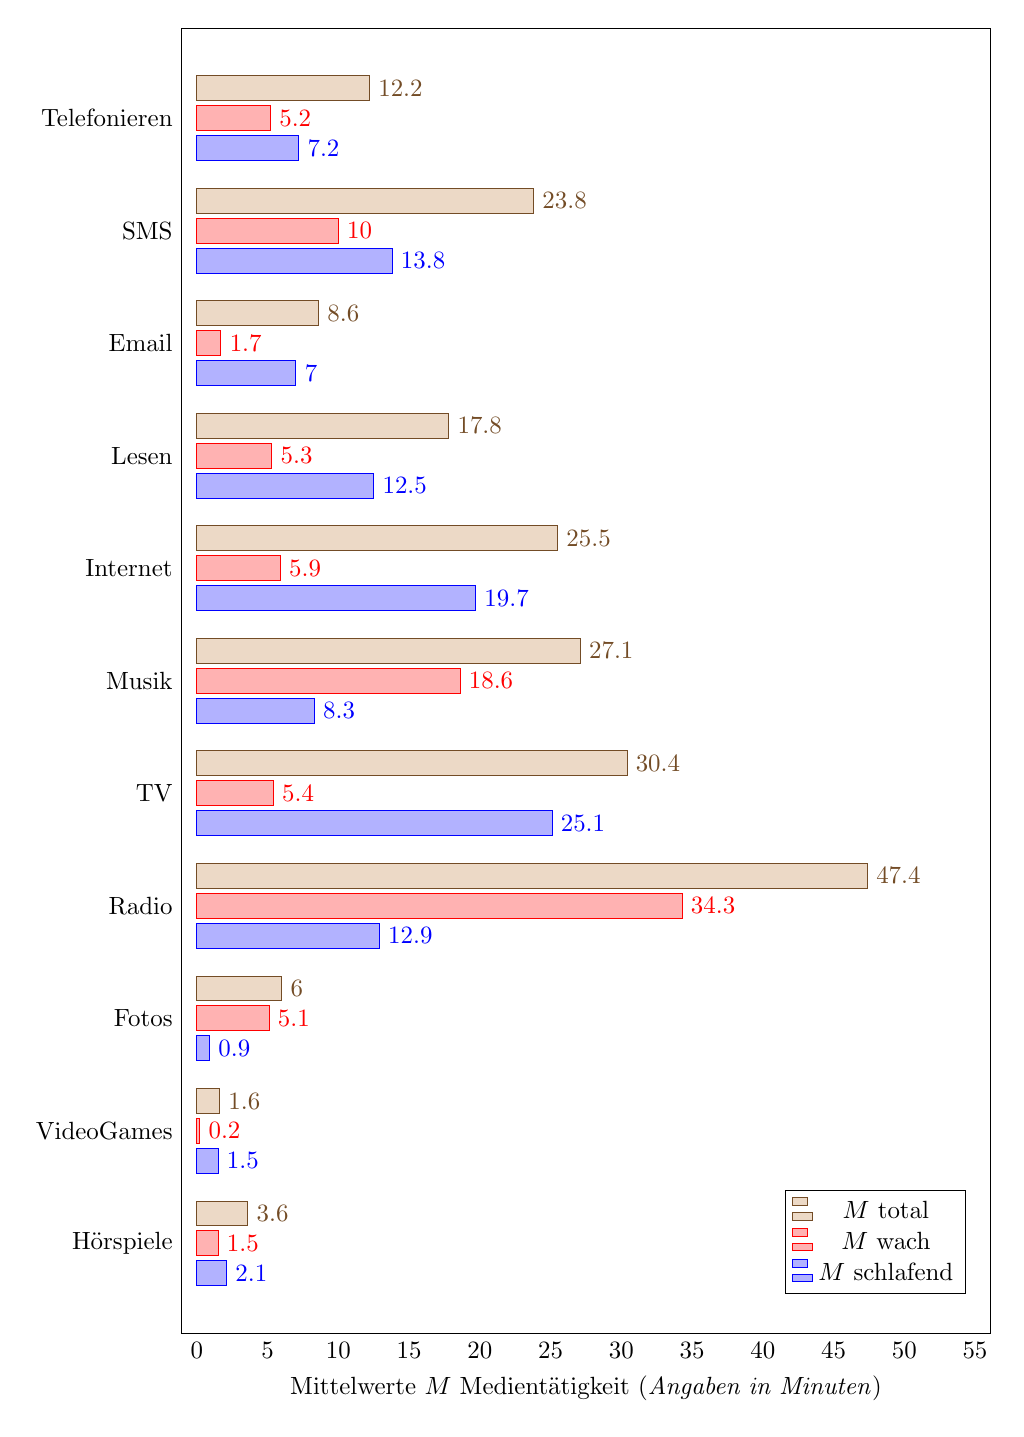
\begin{tikzpicture}[scale=0.9]
  \begin{axis}[
    xbar,
    %y axis line style = { opacity = 0 },
    %axis x line       = none,
    tickwidth         = 0pt,
    xmin              = 0,
    xmax              = 55,
    enlarge y limits  = 0.08,
    enlarge x limits  = 0.02,
    reverse legend,
    legend pos=south east,
    ytick             = data,
    xlabel            = {Mittelwerte $M$ Medientätigkeit (\textit{Angaben in Minuten})},
    height            = 20cm,
    width             = 13cm,
    symbolic y coords = {Hörspiele, VideoGames, Fotos, Radio, TV, Musik, Internet, Lesen, Email, SMS, Telefonieren},
    nodes near coords,
    nodes near coords align={horizontal},
  ]
  %geschlafen
  \addplot coordinates { (7.2,Telefonieren)(13.8,SMS)(7,Email)(12.5,Lesen)(19.7,Internet)(8.3,Musik)(25.1,TV)(12.9,Radio)(0.9,Fotos)(1.5,VideoGames)(2.1,Hörspiele)};
  %wach
  \addplot coordinates { (5.2,Telefonieren)(10,SMS)(1.7,Email)(5.3,Lesen)(5.9,Internet)(18.6,Musik)(5.4,TV)(34.3,Radio)(5.1,Fotos)(.2,VideoGames)(1.5,Hörspiele)};
  %total
  \addplot coordinates { (12.2,Telefonieren)(23.8,SMS)(8.6,Email)(17.8,Lesen)(25.5,Internet)(27.1,Musik)(30.4,TV)(47.4,Radio)(6,Fotos)(1.6,VideoGames)(3.6,Hörspiele)};
  
  \legend{\text{$M$ schlafend}, \text{$M$ wach},  \text{$M$ total}}
  \end{axis}
\end{tikzpicture}
\captionsetup{margin=80pt}
\caption{Medientätigkeit}\label{fig:AppMedientätigkeit}
\end{figure}
